\subsection{Methods}
The denoiser has the very same architecture of the autoencoder presented in Section \ref{sec:aut}.
The only difference is that, before giving the images in input to the encoder we apply to it some random noise. 
Different types of noises can be used, but we implemented a Gaussian noise $\eta \sim \mathcal{N}(\mu, \sigma)$, 
which parameters are gaussianly distributed, i.e. $\mu \sim \mathcal{N}(0, 1)$, $\sigma \sim \mathcal{N}(0.5, 0.5)$.
In this way the network is trained to reconstruct different variations of white noise.
We used the same hyperparameters inferred in Section \ref{sec:aut}.


\subsection{Results}
The denoiser implemented as explained above is performing well, with a test loss of $0.03$. As we can see in Figure \ref{fig:noise} it is able to denoise 
the images in a coherent way, even though with some errors.
\begin{figure}[h]
    \centering
    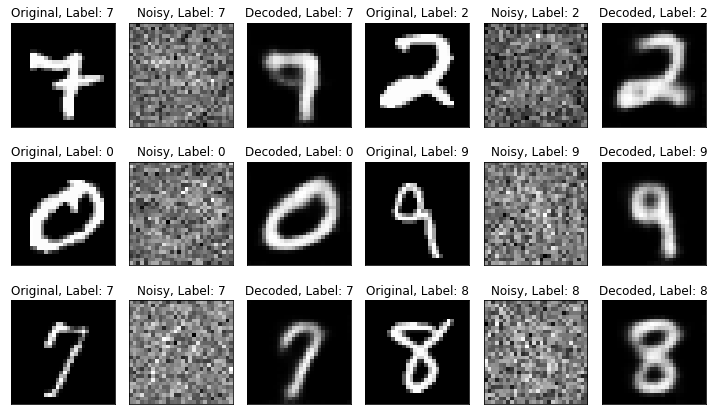
\includegraphics[width=0.8\textwidth]{Images/noise.png}
    \caption{We present the original image, the noisy image and the denoised one for different samples of the test set. The results are really good, even though
    one of the digit is not denoised in the correct way, since it is almost impossible to understand which digit is represented in the noisy image for a 
    human.}
    \label{fig:noise}
\end{figure}